% id: 65-09
% book: 100발100중 3-2 기말 · 01 3-2 기말(원의 성질·통계·부록)
% section: 실전 문제 2회
% figure: crop:fig-65-09.png
% answer: ③
% answer_source: 답지(빠른정답)
% variant_level: 0 (원본 전사)
% 이 파일은 build.mjs 가 items.json 에서 만든다. 고칠 때는 items.json 을 고친다.
\smash{\raisebox{1.5mm}{\dmkichul{100발100중 3-2 기말 65쪽 09번 · 출제유력}}}
다음은 학생 $5$명의 영어 성적에 대한 편차를 조사하여 나타낸 표이다. 이 표에 대한 설명으로 옳지 \underline{않은} 것은?
\par\smallskip\begin{center}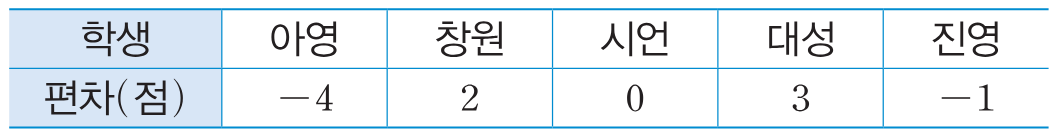
\includegraphics[width=253.4pt]{figures/fig-65-09.png}\end{center}
\begin{choicesv}{\rule[-3ex]{0pt}{8ex}표준편차는 $\sqrt{6}$점이다.}{\rule[-3ex]{0pt}{8ex}시언이의 수학 성적은 평균과 같다.}{\rule[-3ex]{0pt}{8ex}대성과 진영이의 수학 성적의 차는 $2$점이다.}{\rule[-3ex]{0pt}{8ex}수학 성적이 가장 높은 학생은 대성이다.}{\rule[-3ex]{0pt}{8ex}평균이 $72$점이면 아영이의 수학 성적은 $68$점이다.}\end{choicesv}
